\documentclass[xcolor=table]{beamer}
%------------------------------------------------------------
% Theme and Appearance
%------------------------------------------------------------
\usetheme[footline=authorinstitutetitle]{Berlin} 
\setbeamertemplate{navigation symbols}{} 

% Headline with Access Code
\setbeamertemplate{headline}{
    \begin{beamercolorbox}[wd=\paperwidth,ht=2.5ex,dp=1ex,right]{section in head/foot}
        \usebeamerfont{section in head/foot}
        \hspace{0.5cm}
        \ifnum\insertframenumber<30
            \raisebox{-1pt}[0pt][0pt]{\normalsize\textbf{Attendance Code: 079118}}
        \fi
        \hspace{0.5cm}
    \end{beamercolorbox}
}
% Footline with page numbers
\setbeamertemplate{footline}{
    \leavevmode%
    \hbox{%
        \begin{beamercolorbox}[wd=.333333\paperwidth,ht=2.25ex,dp=1ex,left]{author in head/foot}%
            \usebeamerfont{author in head/foot}\hspace*{0.5em}\insertshortauthor
        \end{beamercolorbox}%
        \begin{beamercolorbox}[wd=.333333\paperwidth,ht=2.25ex,dp=1ex,center]{title in head/foot}%
            \usebeamerfont{title in head/foot}\insertshorttitle
        \end{beamercolorbox}%
        \begin{beamercolorbox}[wd=.333333\paperwidth,ht=2.25ex,dp=1ex,right]{date in head/foot}%
            \usebeamerfont{date in head/foot}\insertshortdate{}\hspace*{2em}
            \insertframenumber{} / \inserttotalframenumber\hspace*{2ex} 
        \end{beamercolorbox}}%
    \vskip0pt%
}
\usepackage[utf8]{inputenc}
\usepackage[table]{xcolor}
\usepackage{colortbl}
\usepackage{minted}
\usepackage{lmodern}
\usepackage{tgheros}
\usepackage{hyperref}
\usepackage{tikz}
\usetikzlibrary{shapes, arrows, arrows.meta, positioning, shadows, fit, calc, shapes.multipart}

\renewcommand*\familydefault{\sfdefault}

% Agenda at the start of every section
\AtBeginSection[]
{
    \begin{frame}
        \frametitle{Agenda}
        \tableofcontents[currentsection]
    \end{frame}
}

%------------------------------------------------------------
% Title Page Information
%------------------------------------------------------------
\title[CMP9134 - Week 6]{HCI \& Design Thinking}
\subtitle{CMP9134: Software Engineering}
\author[Francesco Del Duchetto]{Dr Francesco Del Duchetto\\Lecturer in Robotics and Autonomous Systems}
\institute[University of Lincoln]{University of Lincoln}
\date{13 March 2026}

%------------------------------------------------------------
\begin{document}

%--- TITLE FRAME ---
\begin{frame}
    \titlepage
\end{frame}

%--- AGENDA FRAME ---
\begin{frame}
    \frametitle{Today's Agenda}
    \tableofcontents
\end{frame}

%------------------------------------------------------------
\section{Recap: Week 5}
%------------------------------------------------------------

\begin{frame}
    \frametitle{Recap: Architecture \& Software Reuse}
    Last week, we moved from abstract models to system architecture and implementation strategies.
    
    \begin{itemize}
        \item \textbf{Architectural Patterns:} High-level organization of the system (e.g., MVC, Layered architecture).
        \item \textbf{Design Patterns:} Low-level, reusable solutions to common coding problems (e.g., Singleton, Facade, Observer).
        \item \textbf{Component-Based Software Engineering (CBSE):} Building systems by composing independent, standard components.
        \item \textbf{Software Reuse:} The benefits and LEPSI/legal risks of reusing Open Source libraries and copyleft licenses.
    \end{itemize}
\end{frame}

\begin{frame}
    \frametitle{Today's Learning Objectives}
    By the end of this lecture, you should be able to:
    \begin{enumerate}
        \item \textbf{Define} Human-Computer Interaction (HCI) and explain its critical importance in software engineering.
        \item \textbf{Apply} the principles of Design Thinking and User-Centred Design (UCD) to software development.
        \item \textbf{Evaluate} interfaces using cognitive frameworks (Norman, Shneiderman, Fitts's Law).
        \item \textbf{Identify} common prototyping and usability evaluation methods.
        \item \textbf{Analyze} the impact of emerging technologies like AR, VR, and Robotics (HRI) on user experience.
    \end{enumerate}
\end{frame}

%------------------------------------------------------------
\section{Introduction to HCI}
%------------------------------------------------------------

\begin{frame}
    \frametitle{What is Human-Computer Interaction (HCI)?}
    \begin{block}{Definition}
        HCI is the study of how people interact with computers and how to design computer systems that are effective, efficient, and satisfying for people to use.
    \end{block}
    
    \vspace{0.3cm}
    It is a multidisciplinary field that sits at the intersection of:
    \begin{itemize}
        \item \textbf{Computer Science:} The technology, interfaces, and algorithms.
        \item \textbf{Cognitive Science \& Psychology:} Understanding human capabilities, memory, emotions, and mental models.
        \item \textbf{Design / Human Factors:} Ergonomics, accessibility, and visual hierarchy.
    \end{itemize}
\end{frame}

\begin{frame}
    \frametitle{History of HCI}
    HCI has evolved significantly since its inception in the 1980s. The term was popularised by: \textit{Card, Newell, and Moran - The Psychology of Human–Computer Interaction (1983)}.
    
    \vspace{0.2cm}
    \begin{itemize}
        \item \textbf{Early Days (1980s):} Focus on command-line interfaces and basic usability.
        \item \textbf{GUI Era (1990s):} Introduction of graphical user interfaces and desktop environments.
        \item \textbf{Web Age (2000s):} Emphasis on web-based applications and responsive design.
        \item \textbf{Mobile \& Social (2010s):} Adaptation to mobile devices and social media integration.
        \item \textbf{Emerging Trends (2020s):} Integration of AI, AR/VR, and Internet of Things (IoT).
    \end{itemize}
\end{frame}

\begin{frame}
    \frametitle{The Cost of Bad Design}
    Poor design doesn't just frustrate users; it can cause catastrophic financial and safety failures.
    
    \vspace{0.2cm}
    \textbf{Real-World Software Disasters:}
    \begin{itemize}
        \item \textbf{Mars Climate Orbiter (\$125m):} Lost due to a unit conversion error hidden by a poor interface and lack of team communication.
        \item \textbf{Knight Capital Group (\$440m):} Lost in just 45 minutes because a confusing trading interface allowed traders to execute massive orders on outdated software.
        \item \textbf{AT\&T Billing System (\$1bn):} Plagued with interface problems that prevented basic customer requests.
        \item \textbf{Miss Universe 2015:} The host announced the wrong winner because the text hierarchy on the results card was fundamentally flawed.
    \end{itemize}
\end{frame}

\begin{frame}
    \frametitle{Miss Universe 2015: Case study}
    \textbf{Which one is the winner?}
    %side by side original image and a redesigned version but shown one at a time
    \begin{columns}
        \column{0.6\textwidth}
        \begin{center}
            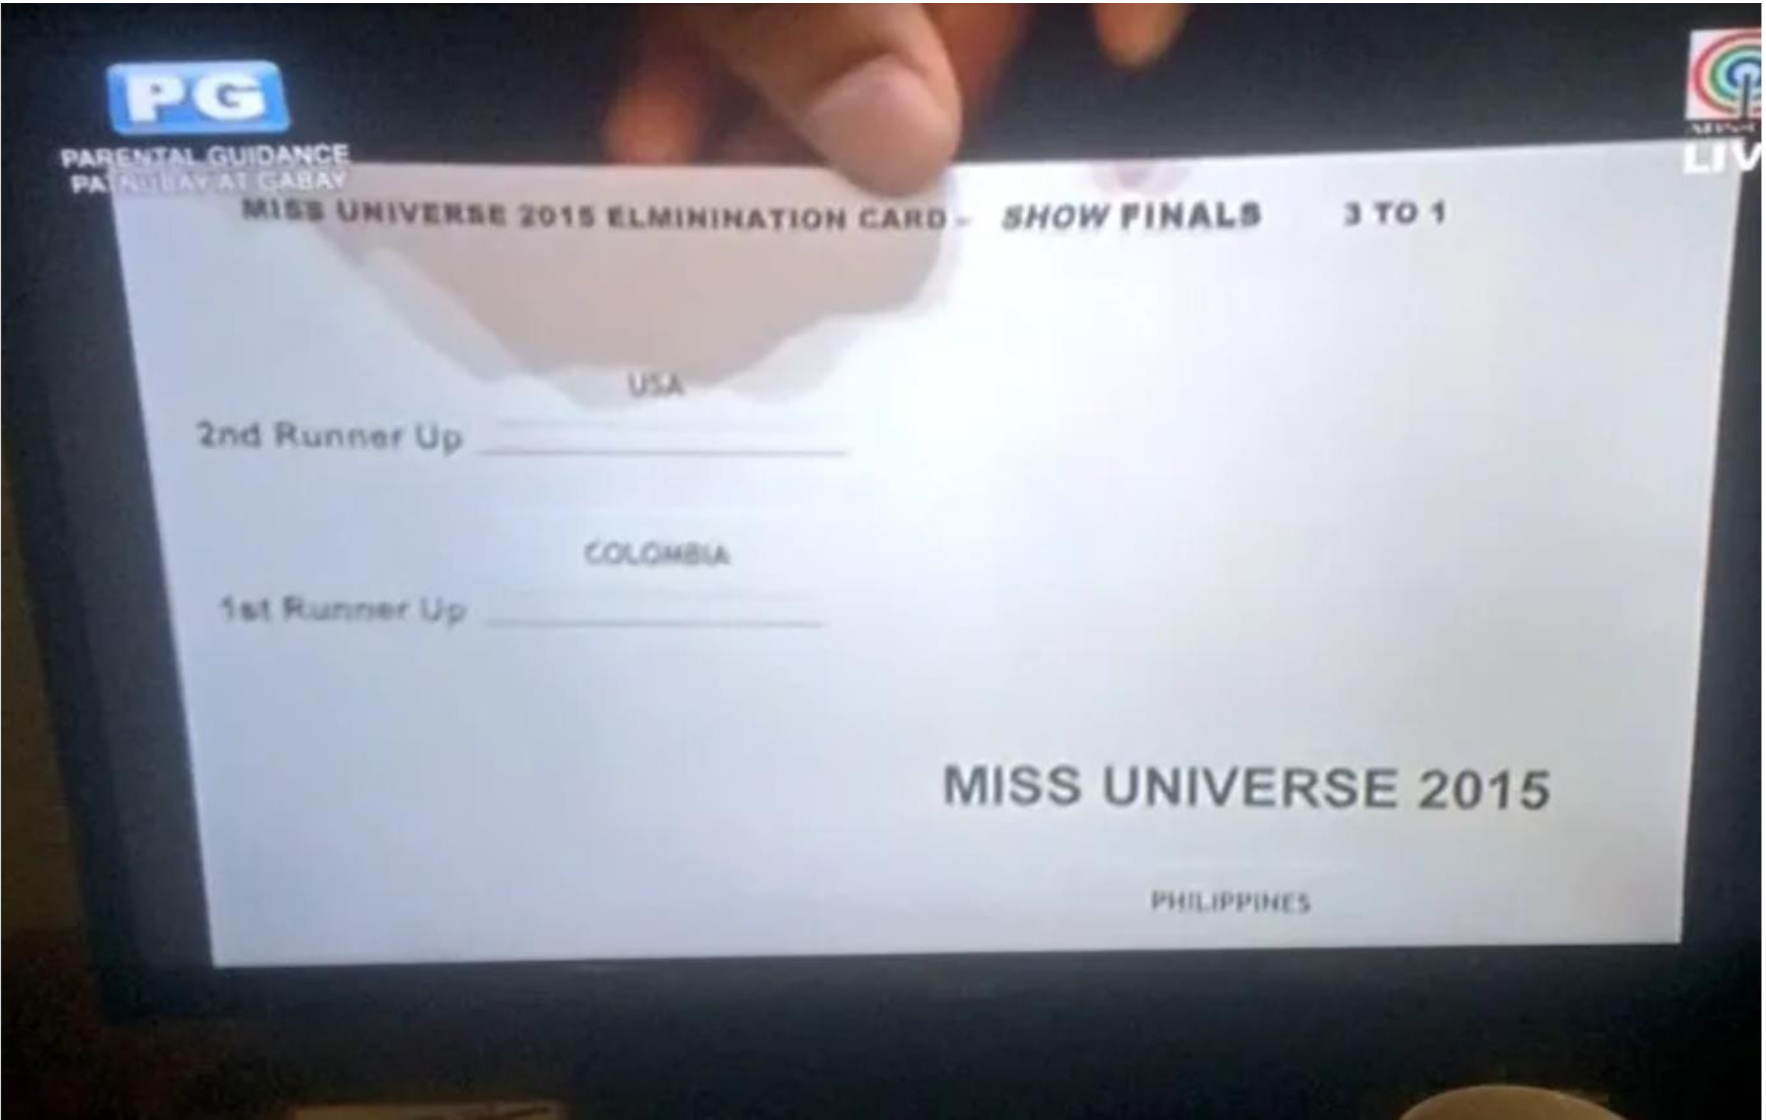
\includegraphics[width=1\textwidth]{imgs/original.png}
            % \captionof{figure}{The original results card.}
        \end{center}
        \pause
        \column{0.6\textwidth}
        \begin{center}
            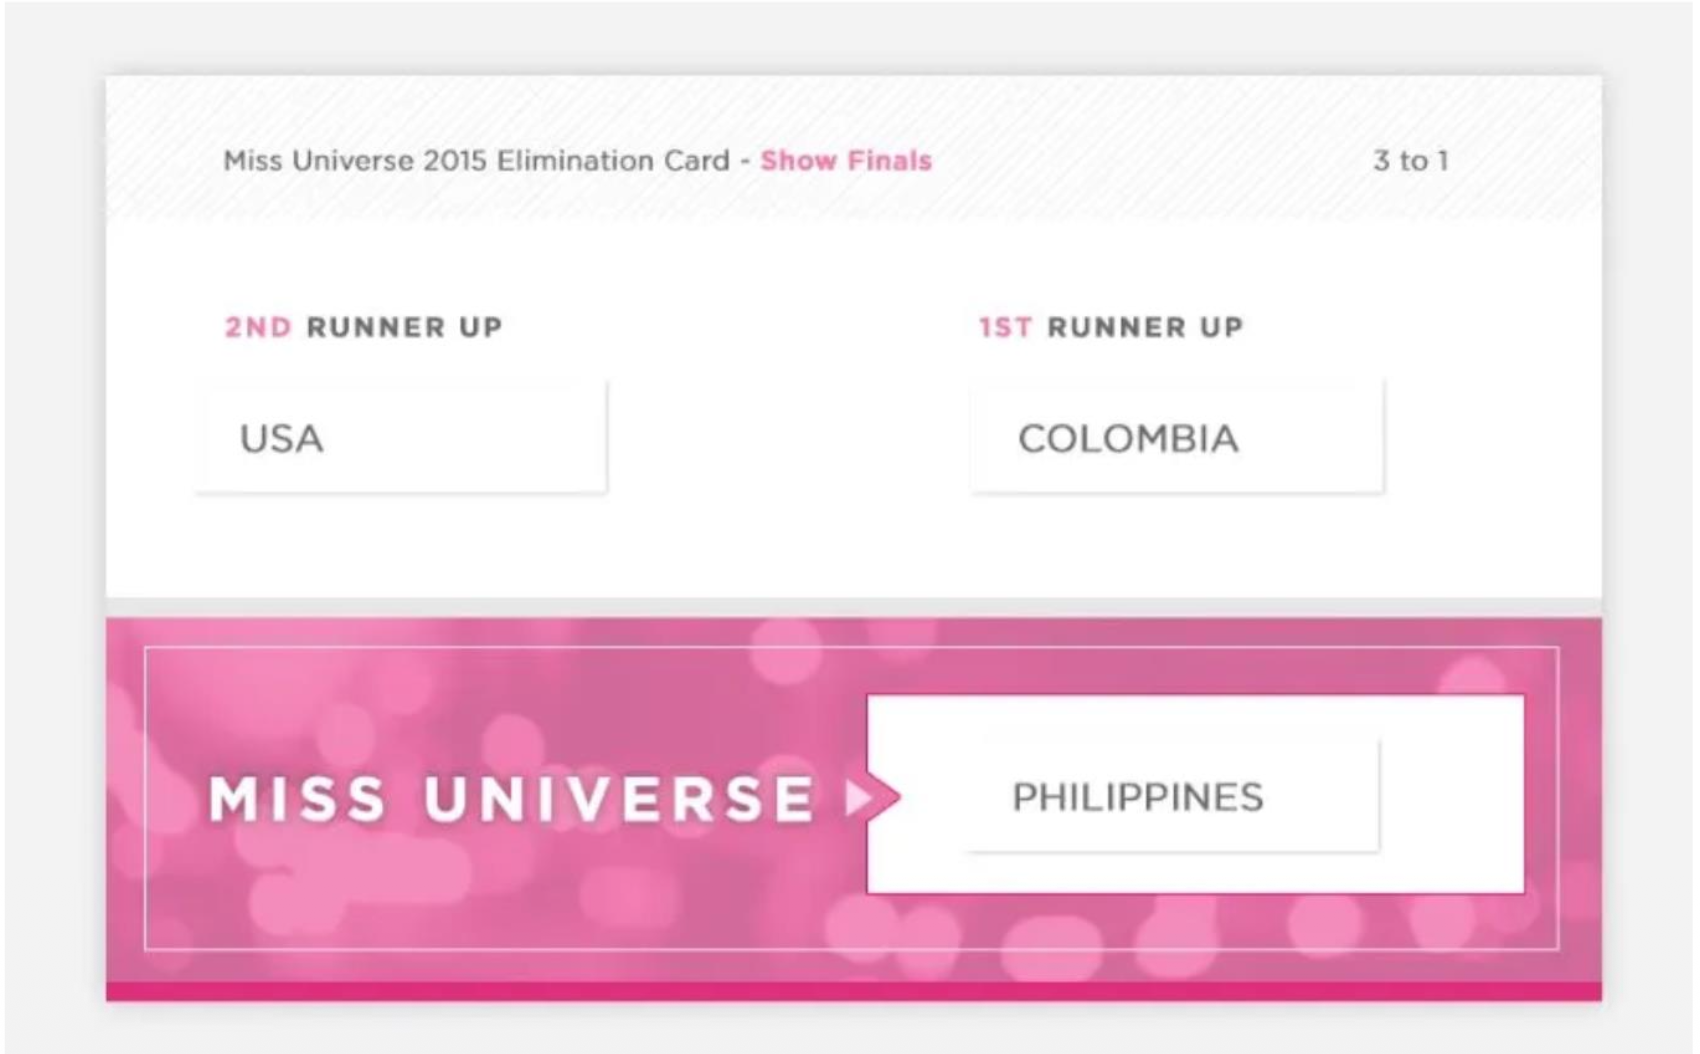
\includegraphics[width=1\textwidth]{imgs/redesigned.png}
            % \captionof{figure}{A redesigned version with better visual hierarchy.}
        \end{center}
    \end{columns}
    \vspace{1cm}
    \tiny\textit{Example on the right: Redesigned version with improved visual hierarchy. Credits: \href{https://medium.com/@ericthomas/how-bad-design-wrecked-steve-harvey-s-universe-ecc05587f308}{https://medium.com/@ericthomas/how-bad-design-wrecked-steve-harvey-s-universe-ecc05587f308}}
\end{frame}

\begin{frame}
    \frametitle{Core Goals of HCI}
    To prevent these disasters, HCI focuses on several distinct goals:
    
    \begin{enumerate}
        \item \textbf{Usability:} Ensuring systems are easy to learn, use, and remember.
        \item \textbf{Utility:} Ensuring systems actually support the tasks users want to accomplish.
        \item \textbf{Safety:} Preventing dangerous errors and posing no risk to users.
        \item \textbf{Accessibility:} Ensuring usability for a diverse range of users, including those with disabilities (Tying directly into WCAG and LEPSI standards!).
        \item \textbf{User Experience (UX):} Providing a satisfying, positive emotional and aesthetic experience.
    \end{enumerate}
\end{frame}

%------------------------------------------------------------
\section{Design Thinking \& UCD}
%------------------------------------------------------------

\begin{frame}[fragile]
    \frametitle{Components of Interaction}
    \small
    Every interaction involves three distinct components. Design Thinking requires us to map all three perfectly.
    
    \vspace{0.1cm}
    \centering
    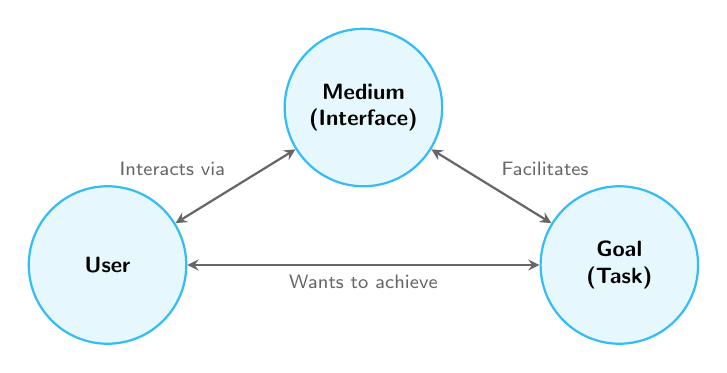
\begin{tikzpicture}[
        node style/.style={circle, draw=cyan!80, fill=cyan!10, thick, minimum size=2cm, align=center, font=\footnotesize\bfseries},
        arrow/.style={<->, >=stealth, thick, gray!80!black}
    ]
        \node[node style] (user) at (0,0) {User};
        \node[node style] (interface) at (3.25,2) {Medium\\(Interface)};
        \node[node style] (task) at (6.5,0) {Goal\\(Task)};
        
        \draw[arrow] (user) -- (interface) node[midway, above left, font=\scriptsize] {Interacts via};
        \draw[arrow] (interface) -- (task) node[midway, above right, font=\scriptsize] {Facilitates};
        \draw[arrow] (user) -- (task) node[midway, below, font=\scriptsize] {Wants to achieve};
    \end{tikzpicture}
    
    \vspace{0.1cm}
    \begin{itemize}
        \item \textbf{User:} Capabilities, experience, emotions.
        \item \textbf{Task:} The complexity and time required to achieve the goal.
        \item \textbf{Medium:} The graphical/hardware interface. \textit{For users, the interface IS the program!}
    \end{itemize}
\end{frame}

\begin{frame}
    \frametitle{The Evolution of Design Thinking}
    Before we look at the modern process, where did "Design Thinking" come from?
    
    \begin{itemize}
        \item \textbf{1969 - Cognitive Foundations:} Nobel laureate Herbert Simon published \textit{The Sciences of the Artificial}, introducing the idea of "design" as a formal way of thinking and problem-solving.
        \item \textbf{1980s \& 90s - User-Centered Design:} Architecture, engineering, and computer science began moving away from purely technical problem-solving to human-centered problem-solving.
        \item \textbf{2000s - Mainstream Adoption:} The design firm \textbf{IDEO} (founded by David Kelley) and the \textbf{Stanford d.school} formalized the process. They proved it could be applied to business, software, and services, not just physical hardware.
    \end{itemize}
\end{frame}

\begin{frame}
    \frametitle{What exactly is Design Thinking?}
    \begin{block}{A Human-Centered Approach}
        Design Thinking is a non-linear, iterative process that teams use to understand users, challenge assumptions, redefine problems, and create innovative solutions to prototype and test.
    \end{block}
    
    \vspace{0.3cm}
    \textbf{It tackles "Wicked Problems":}
    \begin{itemize}
        \item A "wicked problem" is one that is ill-defined, tricky, or lacks a clear right/wrong answer (e.g., "How do we make remote collaboration feel natural?").
        \item Standard engineering asks: \textit{"How do we build this feature?"}
        \item Design thinking asks: \textit{"Is this the right feature to build for this user?"}
    \end{itemize}
\end{frame}

\begin{frame}
    \frametitle{Why Design Thinking in Software Engineering?}
    Historically, software engineering was heavily driven by hardware limitations and strict feature lists. 
    
    \vspace{0.3cm}
    \textbf{The problem with Feature-Driven Development:}
    \begin{itemize}
        \item \textbf{Feature Creep:} Adding more buttons, menus, and tools simply because the technology allows it, not because the user needs it.
        \item \textbf{The Engineer's Bias:} The false assumption that the end-user understands the system's architecture the same way the engineer does.
    \end{itemize}
    
    \vspace{0.3cm}
    \textbf{The Design Thinking Solution:}
    By empathizing with the user \textit{before} writing any code, software engineers avoid the costly mistake of spending months building a robust, bug-free system that nobody actually wants to use.
\end{frame}

\begin{frame}[fragile]
    \frametitle{Design Thinking: The Process}
    User-Centred Design (UCD) is an approach that places the needs and goals of users at the absolute forefront. Today, this is widely standardized as \textbf{Design Thinking}.
    
    \vspace{0.3cm}
    \centering
    \resizebox{\textwidth}{!}{
    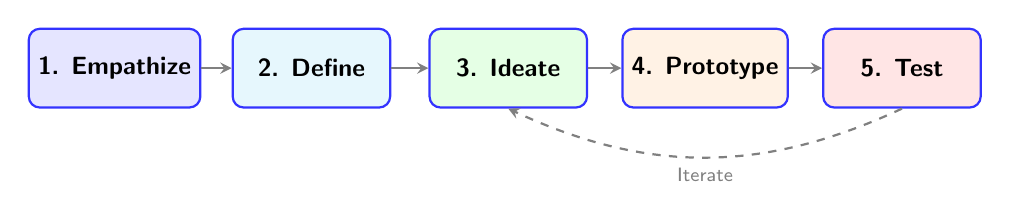
\begin{tikzpicture}[
        stage/.style={rectangle, draw=blue!80, fill=white, thick, rounded corners, minimum width=2cm, minimum height=1cm, align=center, font=\small\bfseries},
        arrow/.style={->, >=stealth, thick, gray}
    ]
        \node[stage, fill=blue!10] (emp) at (0,0) {1. Empathize};
        \node[stage, fill=cyan!10] (def) at (2.5,0) {2. Define};
        \node[stage, fill=green!10] (ide) at (5,0) {3. Ideate};
        \node[stage, fill=orange!10] (pro) at (7.5,0) {4. Prototype};
        \node[stage, fill=red!10] (tes) at (10,0) {5. Test};
        
        \draw[arrow] (emp) -- (def);
        \draw[arrow] (def) -- (ide);
        \draw[arrow] (ide) -- (pro);
        \draw[arrow] (pro) -- (tes);
        \draw[arrow, dashed] (tes.south) to[bend left=25] node[midway, below, font=\scriptsize] {Iterate} (ide.south);
    \end{tikzpicture}
    }
    
    \vspace{0.3cm}
    \begin{itemize}
        \item \textbf{Empathize:} Understand the users (Surveys, Observations).
        \item \textbf{Define:} Specify their core problems and goals (Task Analysis).
        \item \textbf{Ideate:} Generate guidelines, principles, and architectures.
        \item \textbf{Prototype:} Build cheap, interactive simulations.
        \item \textbf{Test:} Evaluate the prototypes with real users.
    \end{itemize}
\end{frame}

%------------------------------------------------------------
\section{HCI Principles \& Laws}
%------------------------------------------------------------

\begin{frame}
    \frametitle{Shneiderman's Eight Golden Rules}
    When Ideating, we follow established cognitive rules. Ben Shneiderman in 1986 consolidated UI design into eight general heuristics:
    \small
    \begin{enumerate}
        \item \textbf{Strive for consistency:} Identical terminology, colors, and layout.
        \item \textbf{Enable shortcuts:} For frequent users (e.g., Ctrl+C).
        \item \textbf{Offer informative feedback:} For every user action.
        \item \textbf{Design dialogs to yield closure:} Let users know a task is done.
        \item \textbf{Offer simple error handling:} Prevent errors before they occur.
        \item \textbf{Permit easy reversal of actions:} The "Undo" button reduces anxiety.
        \item \textbf{Support internal locus of control:} Make users feel they are in charge.
        \item \textbf{Reduce short-term memory load:} Keep displays simple; don't make users remember things from one screen to the next.
    \end{enumerate}
\end{frame}

\begin{frame}
    \frametitle{Norman's Seven Principles}
    Donald Norman in 1988 proposed principles to transform difficult tasks:
    
    \begin{itemize}
        \item \textbf{Knowledge in the world \& head:} Don't force users to memorize everything; put hints in the UI.
        \item \textbf{Simplify task structures:} Avoid overwhelming cognitive load.
        \item \textbf{Make things visible:} Users should immediately see what actions are possible (\textit{affordances}).
        \item \textbf{Get the mapping right:} Controls should map to their physical/logical outcomes (e.g., a "Volume Up" button should point upwards).
        \item \textbf{Convert constraints into advantages:} Use physical or visual constraints to prevent illegal actions.
        \item \textbf{Design for error:} Assume users will make mistakes.
        \item \textbf{Standardize:} When all else fails, rely on established standards.
    \end{itemize}
\end{frame}

\begin{frame}
    \frametitle{HCI Laws for Software Engineers}
    Beyond general principles, two scientific laws dictate how we build interfaces:
    
    \vspace{0.3cm}
    \begin{block}{Fitts's Law}
        The time required to rapidly move to a target area is a function of the \textbf{ratio between the distance to the target and the width of the target}.
        \textit{Takeaway: Make important buttons (like "Submit" or "Emergency Stop") large and place them near the user's cursor or thumb.}
    \end{block}
    
    \begin{block}{Hick's Law}
        The time it takes for a person to make a decision increases logarithmically as the \textbf{number of choices increases}.
        \textit{Takeaway: Don't overwhelm users with 50 menu items. Group them logically to reduce decision fatigue.}
    \end{block}
\end{frame}

%------------------------------------------------------------
\section{Prototyping \& Evaluation}
%------------------------------------------------------------

\begin{frame}[fragile]
    \frametitle{Iterative Prototyping Process}
    \begin{center}
        \resizebox{\textwidth}{!}{
        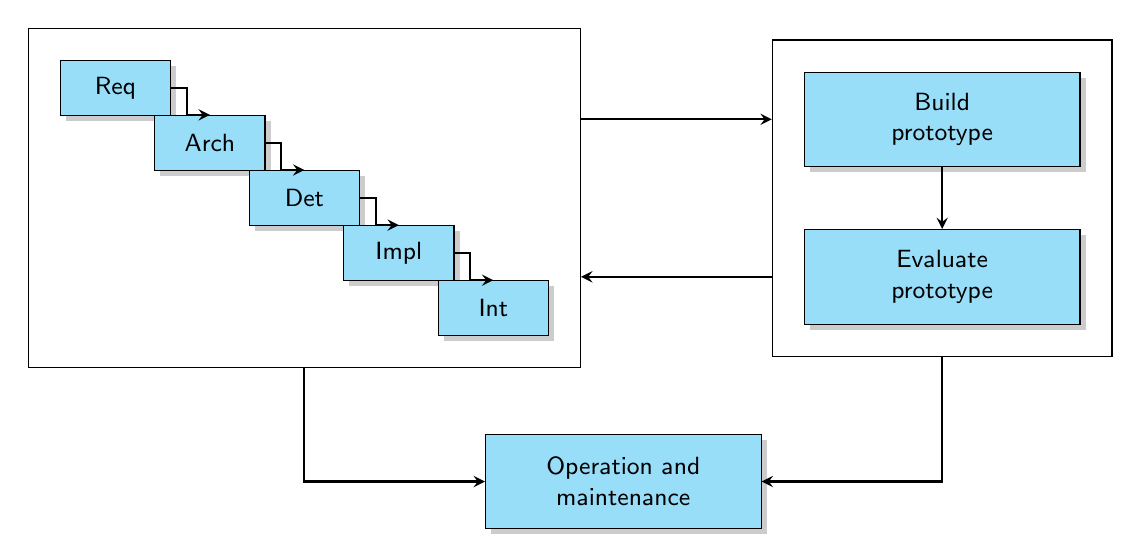
\begin{tikzpicture}[
            box/.style={draw=black, fill=cyan!40, drop shadow={opacity=0.4, shadow xshift=2pt, shadow yshift=-2pt}, minimum height=0.7cm, align=center, font=\small\sffamily},
            smallbox/.style={box, minimum width=1.4cm},
            largebox/.style={box, minimum width=3.5cm, minimum height=1.2cm},
            arr/.style={->, >=stealth, thick},
            groupbox/.style={draw=black, thin, inner sep=0.4cm}
        ]
            % Left Group (Waterfall steps)
            \node[smallbox] (req) at (0, 0) {Req};
            \node[smallbox] (arch) at (1.2, -0.7) {Arch};
            \node[smallbox] (det) at (2.4, -1.4) {Det};
            \node[smallbox] (impl) at (3.6, -2.1) {Impl};
            \node[smallbox] (int) at (4.8, -2.8) {Int};

            \draw[arr] (req.east) -- ++(0.2,0) |- (arch.north);
            \draw[arr] (arch.east) -- ++(0.2,0) |- (det.north);
            \draw[arr] (det.east) -- ++(0.2,0) |- (impl.north);
            \draw[arr] (impl.east) -- ++(0.2,0) |- (int.north);

            \node[groupbox, fit=(req) (int)] (leftgroup) {};

            % Right Group (Prototyping)
            \node[largebox] (build) at (10.5, -0.4) {Build\\prototype};
            \node[largebox] (eval) at (10.5, -2.4) {Evaluate\\prototype};

            \draw[arr] (build.south) -- (eval.north);

            \node[groupbox, fit=(build) (eval)] (rightgroup) {};

            % Bottom Node (Operation)
            \node[largebox] (om) at (6.45, -5.0) {Operation and\\maintenance};

            % Connections between groups
            \coordinate (Lout1) at (leftgroup.east |- build.west);
            \coordinate (Rin1)  at (rightgroup.west |- build.west);
            \draw[arr] (Lout1) -- (Rin1);

            \coordinate (Rout2) at (rightgroup.west |- eval.west);
            \coordinate (Lin2)  at (leftgroup.east |- eval.west);
            \draw[arr] (Rout2) -- (Lin2);

            % Bottom connections
            \draw[arr] (leftgroup.south) |- (om.west);
            \draw[arr] (rightgroup.south) |- (om.east);

        \end{tikzpicture}
        }
    \end{center}
\end{frame}

\begin{frame}
    \frametitle{Types of Prototypes}
    An interactive system cannot be completely specified from the beginning. You must build prototypes before writing production code.
    
    \begin{itemize}
        \item \textbf{GUI Mockups / Wireframes:} Static visual sketches of the interface layout. Can be low-fidelity (paper) or high-fidelity (Figma).
        \item \textbf{Storyboards:} Comic-strip style flows showing how the user interacts with the system contextually over time.
        \item \textbf{Wizard of Oz:} A highly effective technique where the user interacts with a "working" interface, but the backend is secretly operated by a human researcher typing in responses.
    \end{itemize}
\end{frame}

\begin{frame}
    \frametitle{GUI Mockups/Wireframes}

    These can be created using tools like Figma, Balsamiq, or even pen and paper. The key is to focus on layout and flow, not on visual polish.

    \begin{center}
        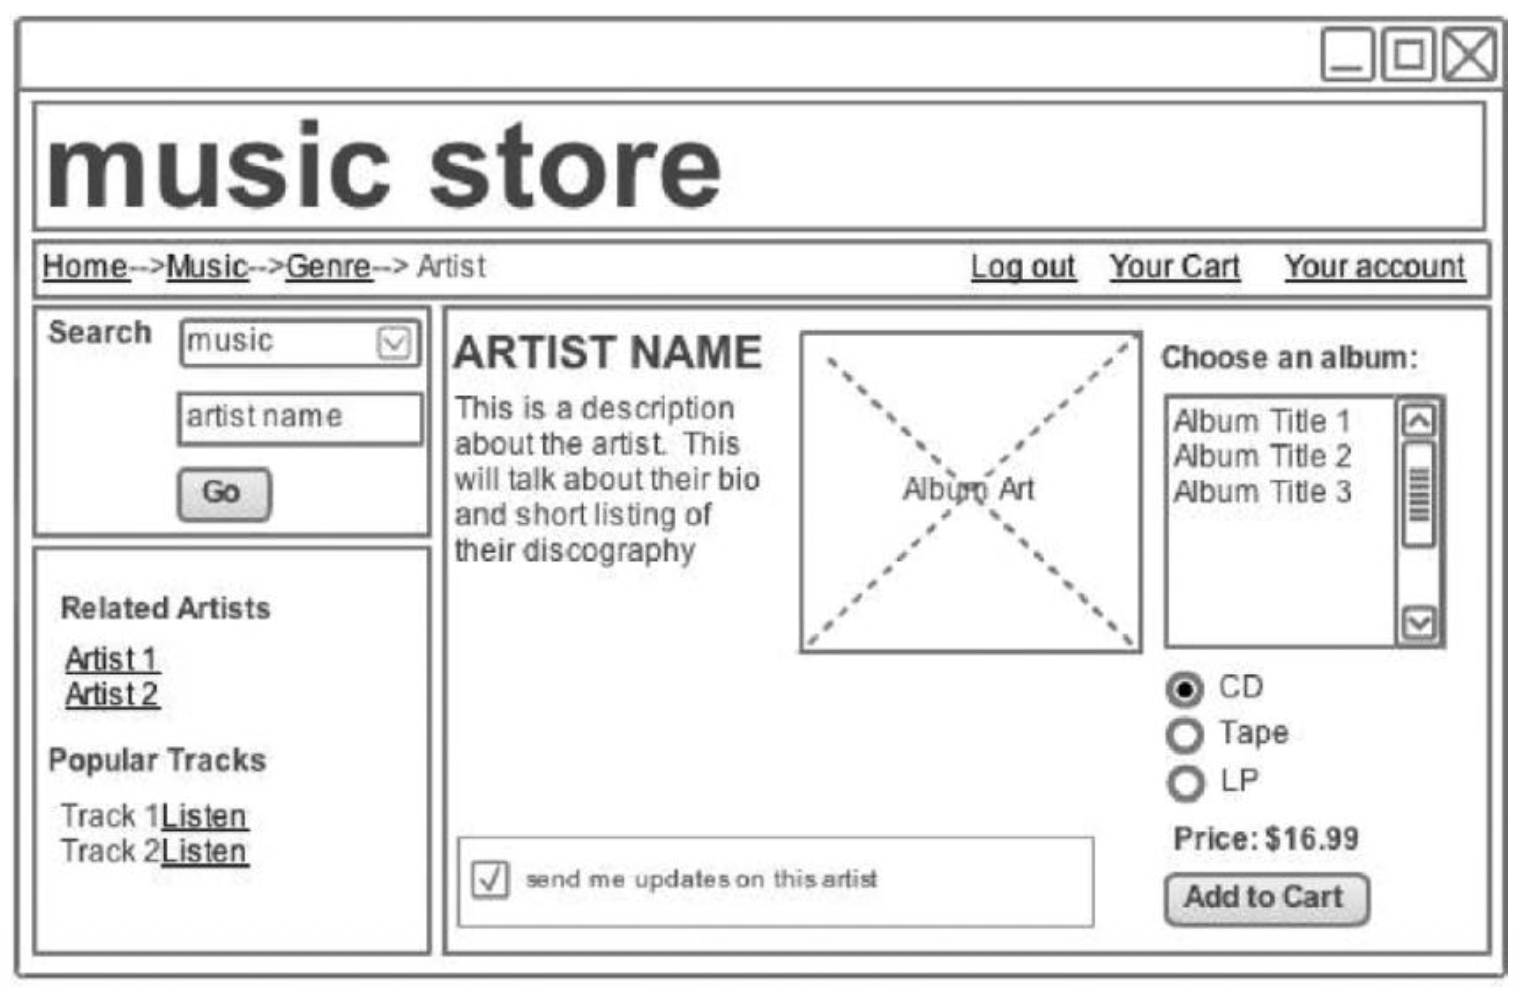
\includegraphics[width=0.8\textwidth]{imgs/GUImockup.png}
        % \captionof{figure}{Example of a high-fidelity wireframe created in Figma.}
    \end{center}

\end{frame}

\begin{frame}
    \frametitle{Storyboards}
    Storyboards are a powerful way to visualize the user's journey through the system, especially for complex interactions that involve multiple steps or contexts.
    
    \begin{center}
        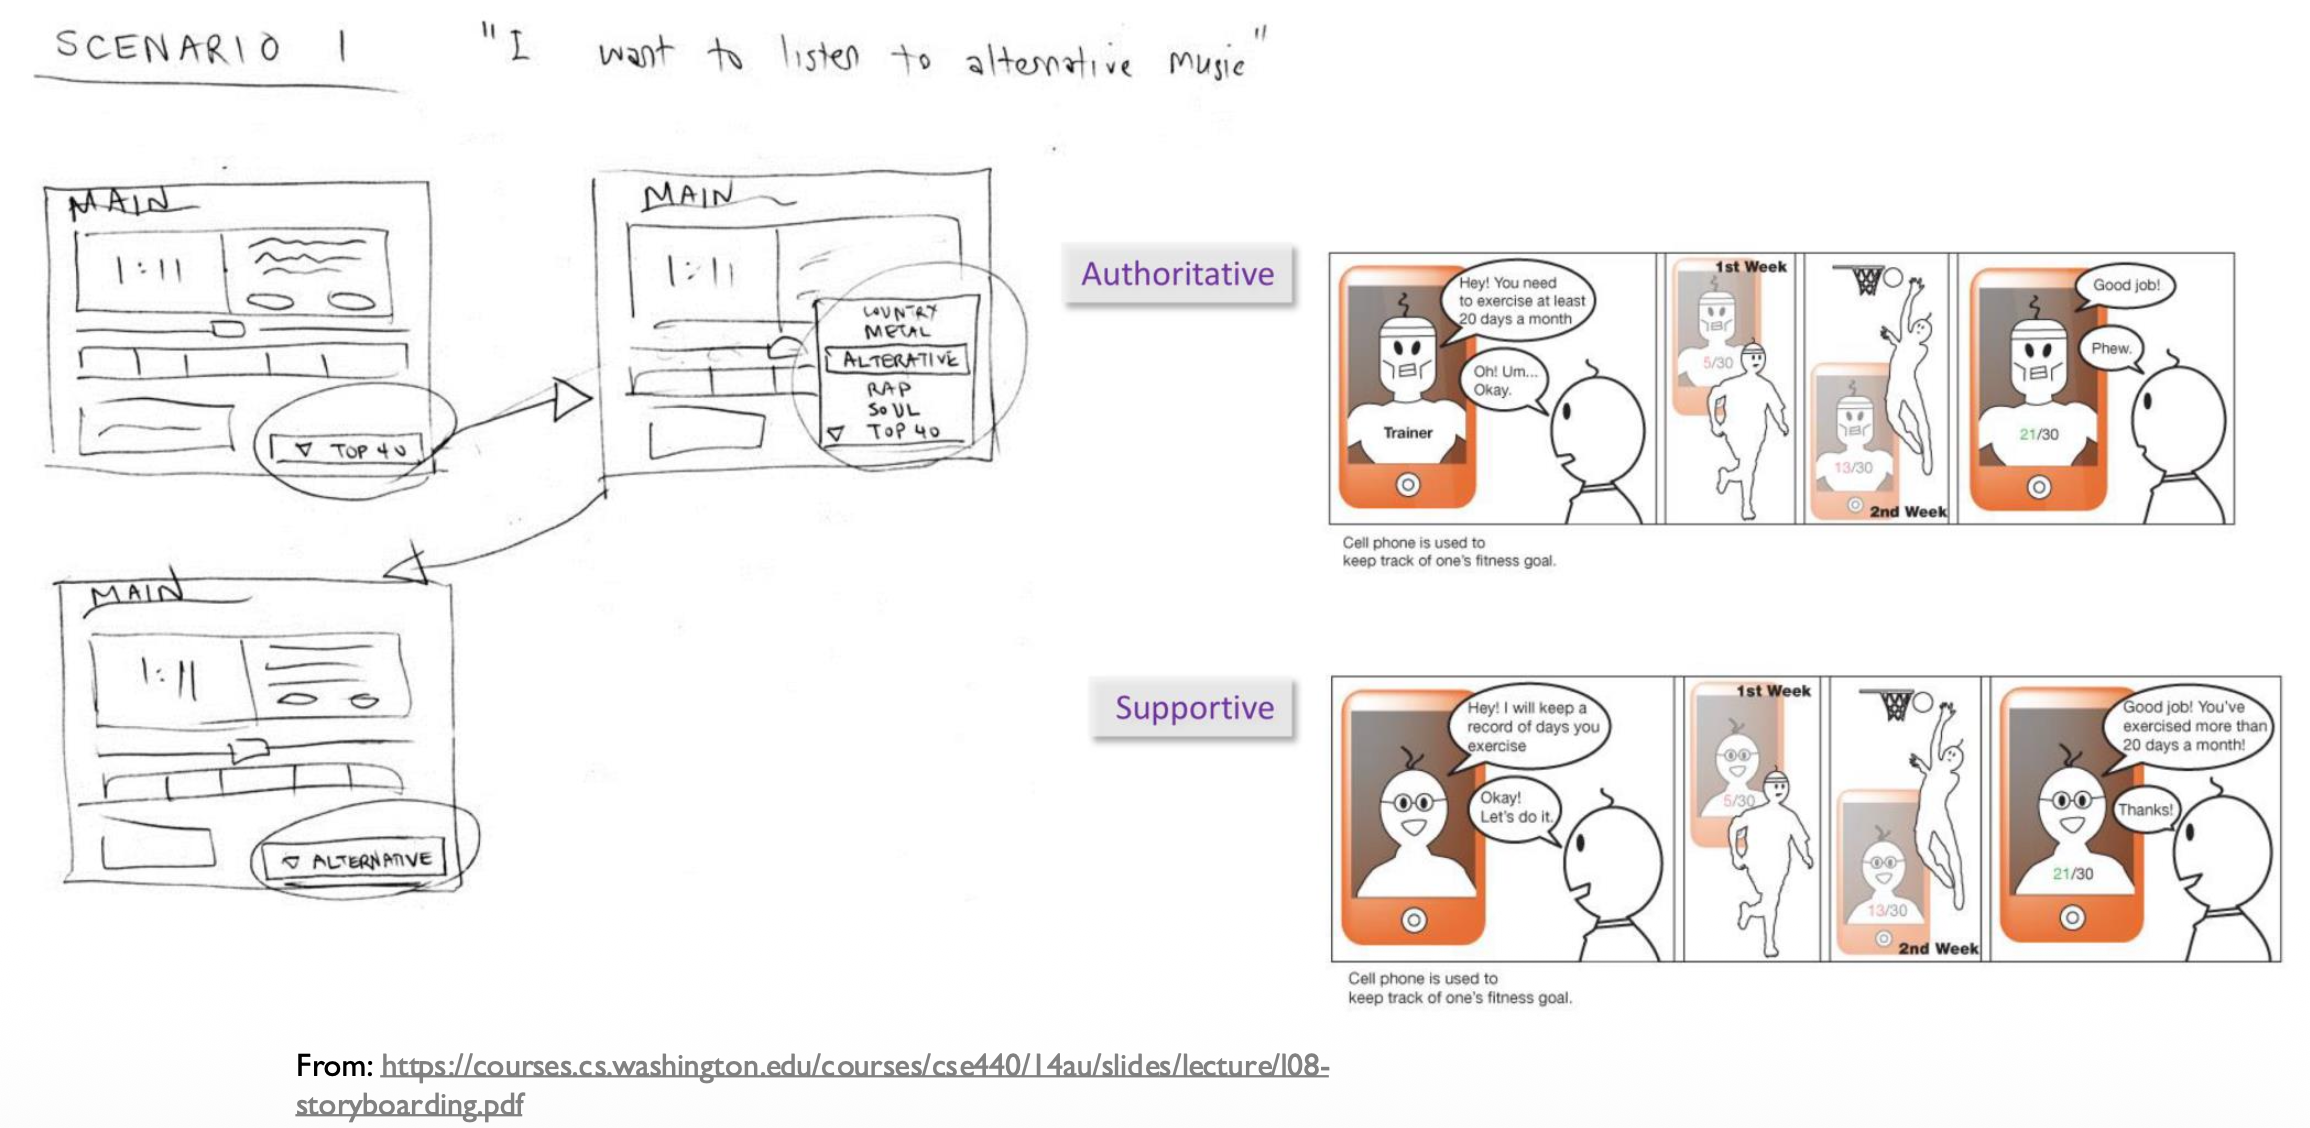
\includegraphics[width=1\textwidth]{imgs/storyboards.png}
        % \captionof{figure}{Example of a storyboard illustrating a user's interaction with a mobile app.}
    \end{center}
\end{frame}

\begin{frame}
    \frametitle{Wizard of Oz}
    This method allows you to test complex interactions (like voice commands or AI responses) without having to build the actual backend logic.
    
    \begin{center}
        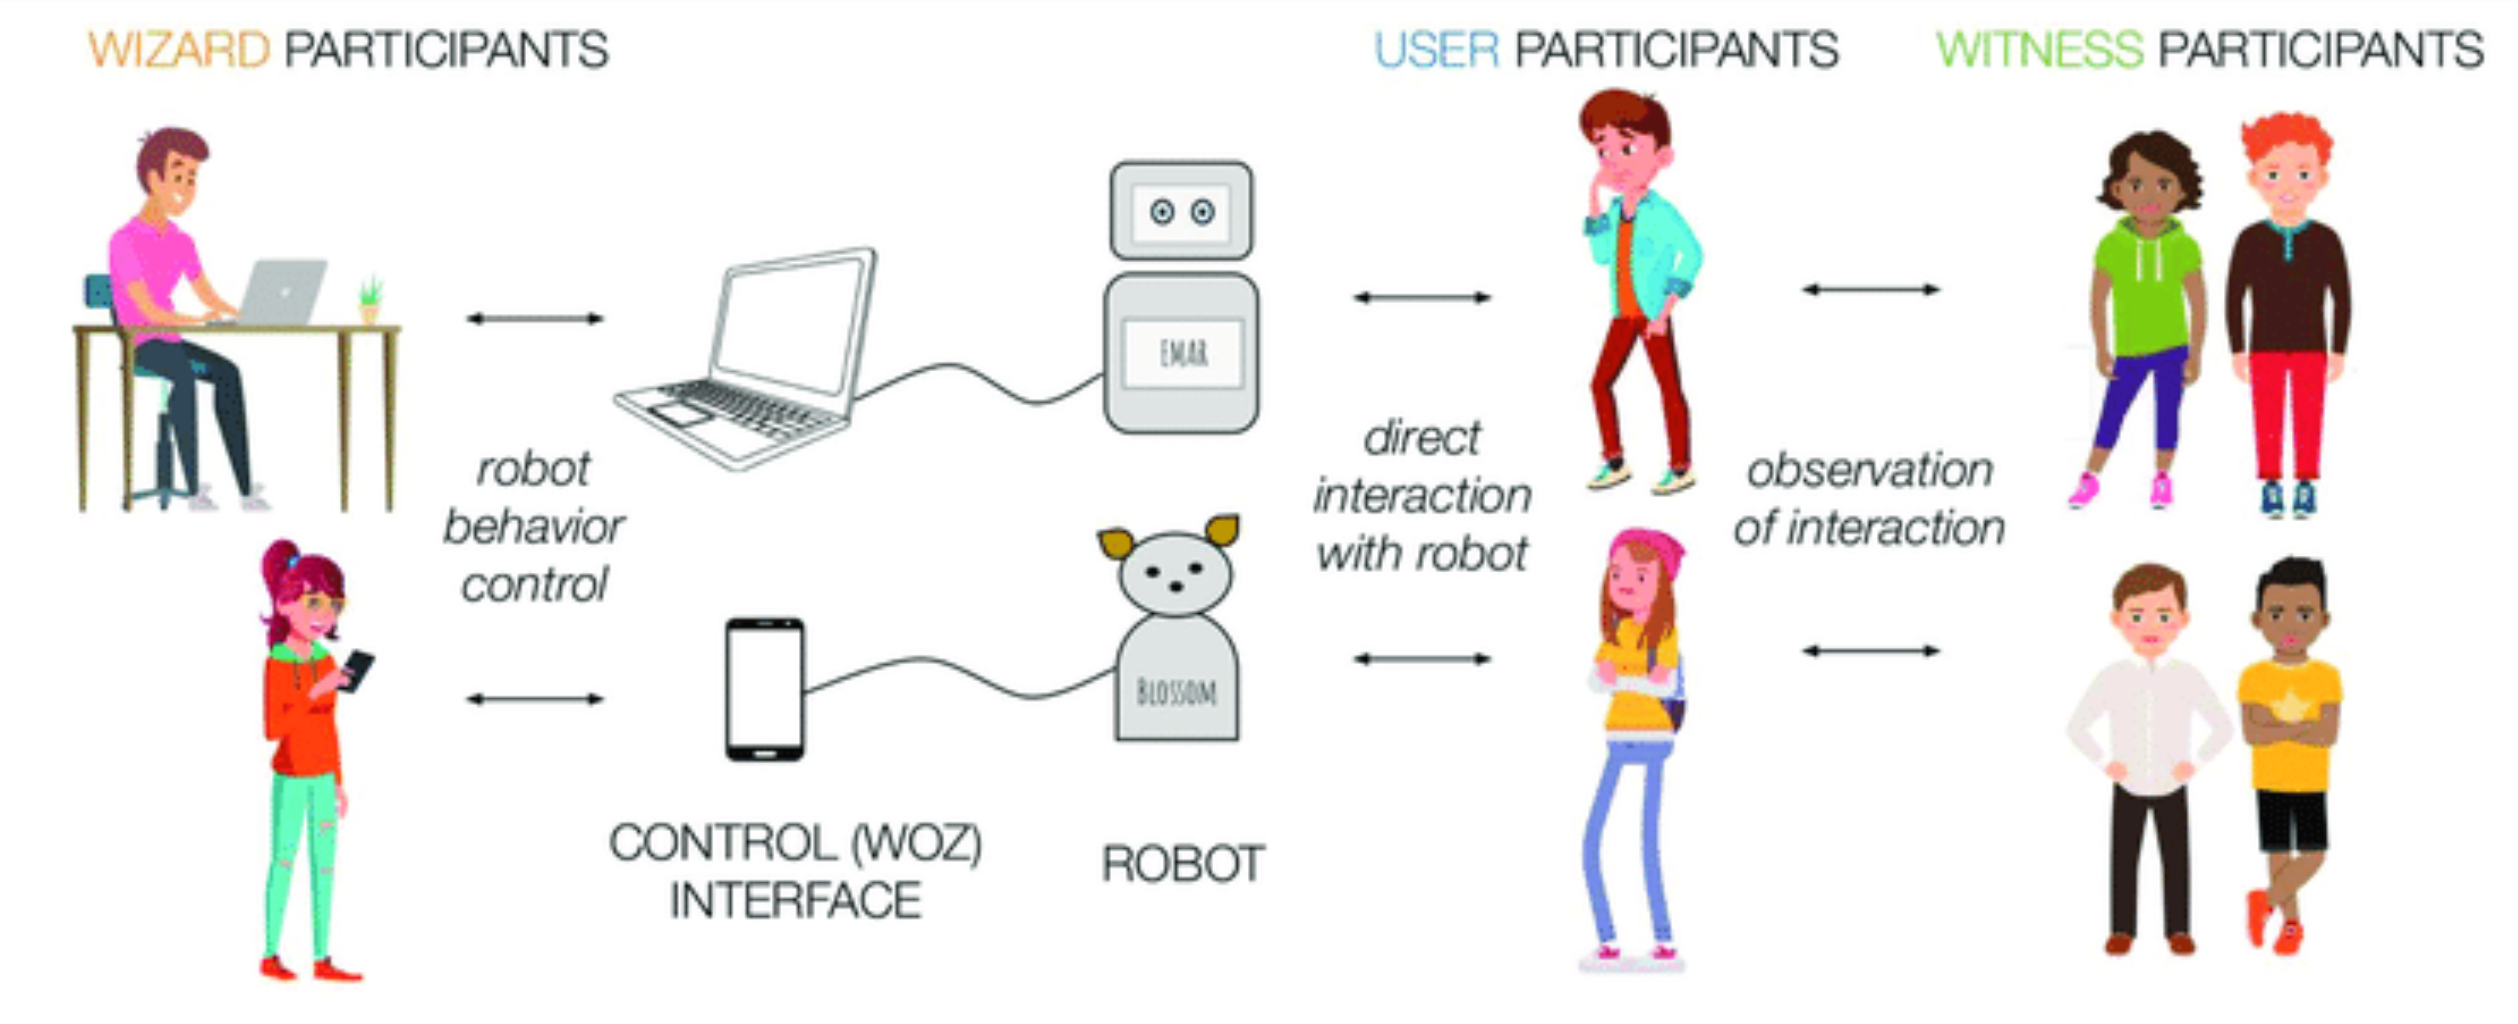
\includegraphics[width=1\textwidth]{imgs/woz.png}
        % \captionof{figure}{In a Wizard of Oz prototype, the user interacts with a seemingly functional interface, while a human operator controls the responses behind the scenes.}
    \end{center}
\end{frame}

\begin{frame}
    \frametitle{Wizard of Oz -- Limited Functionality Simulation}
    \small
    Can simulate interactions difficult/expensive/impossible to implement, such as natural language processing or AI behaviors.
    
    \begin{center}
        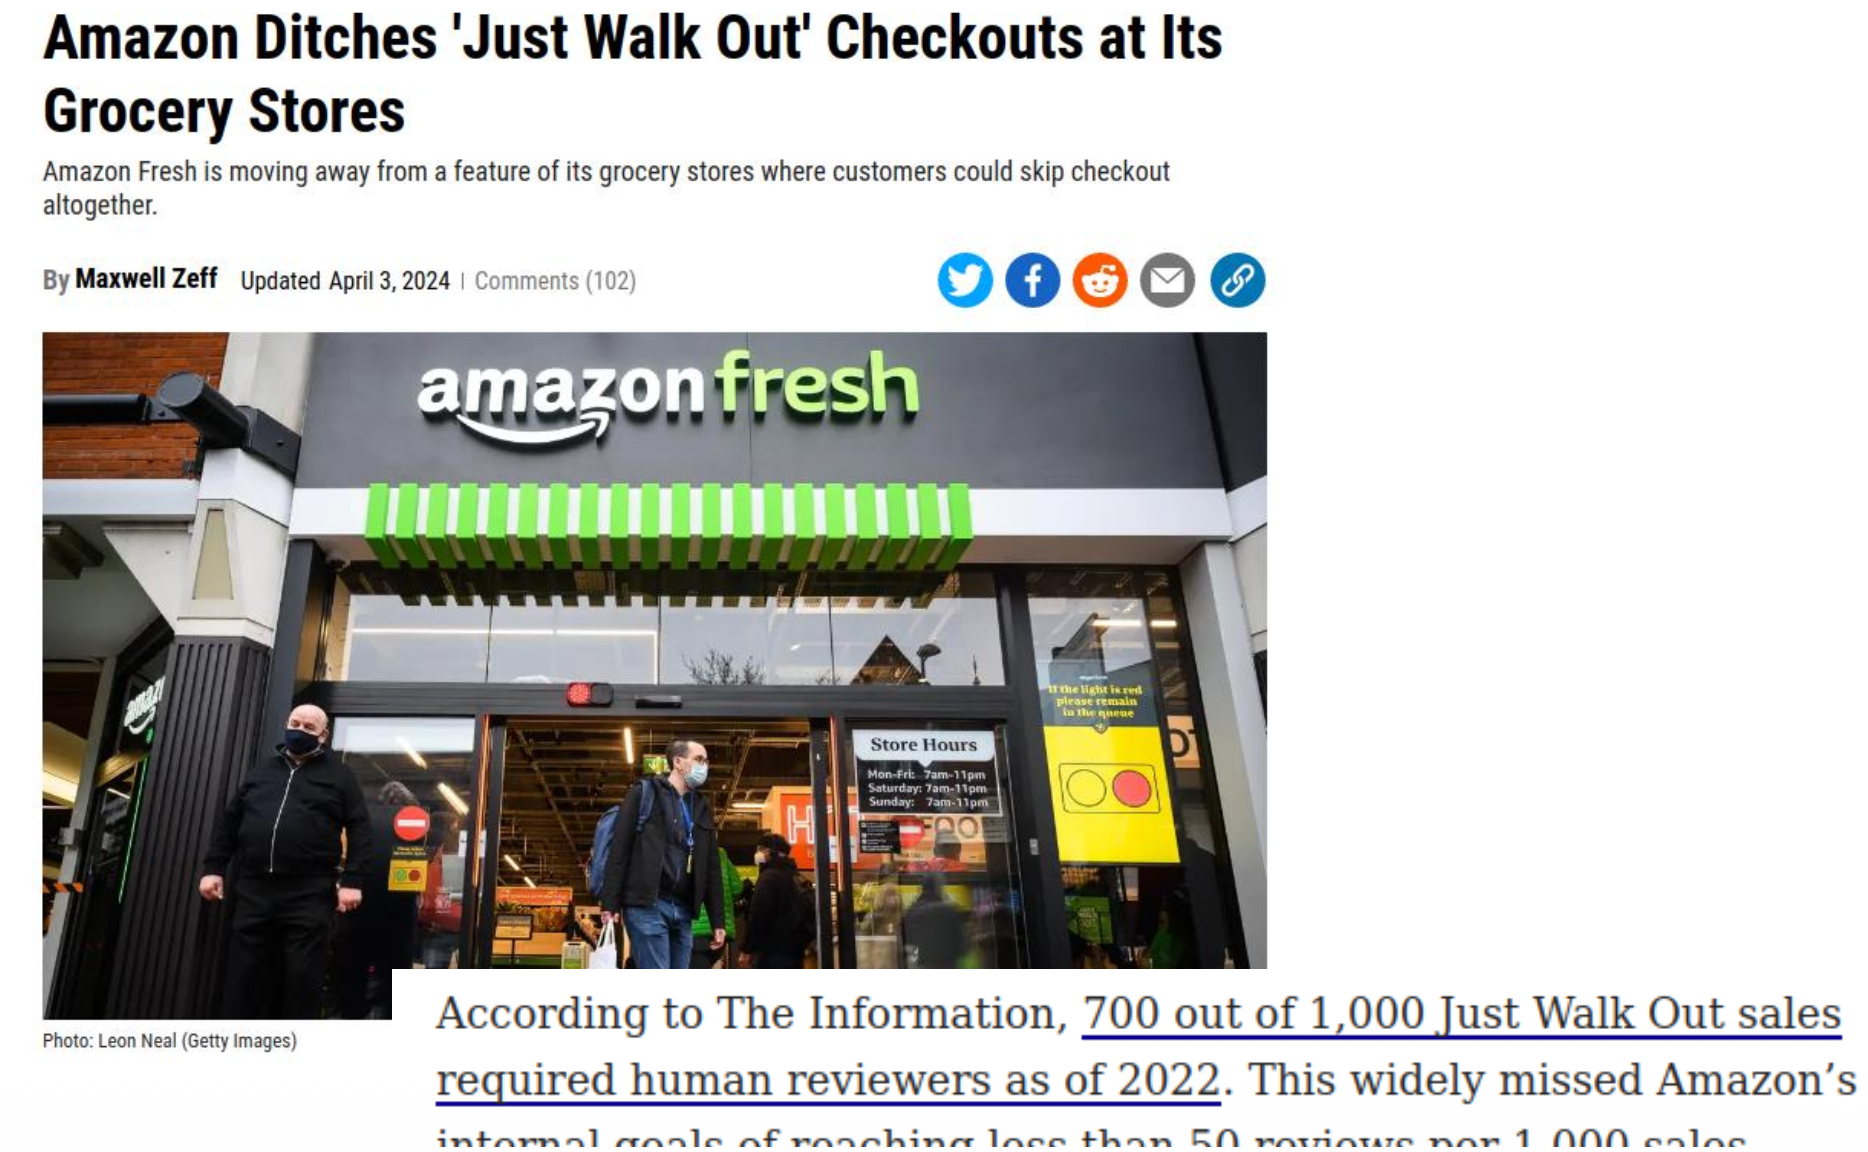
\includegraphics[width=1\textwidth]{imgs/amazon.png}
        % \captionof{figure}{In a Wizard of Oz prototype, the user interacts with a seemingly functional interface, while a human operator controls the responses behind the scenes.}
    \end{center}
\end{frame}

\begin{frame}
    \frametitle{Usability Evaluation Methods}
    How do we know if our prototype is actually good?
    
    \begin{enumerate}
        \item \textbf{User Testing:} Observing actual participants as they attempt to complete predefined tasks. Researchers collect quantitative data (time, errors) and qualitative data (frustration, confusion).
        \item \textbf{Heuristic Evaluation:} A fast, cost-effective method where UI \textit{experts} (not end-users) evaluate the interface against a set of principles (like Shneiderman's rules) to find flaws.
        \item \textbf{Cognitive Walkthrough:} Evaluators step through the tasks, simulating the exact thought process and mental model of a novice user at every click ("Would the user know to click here?").
    \end{enumerate}
\end{frame}

% %------------------------------------------------------------
% \section{User Testing in Practice}
% %------------------------------------------------------------

\begin{frame}
    \frametitle{The Goal of User Testing}
    While Heuristic Evaluations and Cognitive Walkthroughs rely on experts, \textbf{User Testing} puts your prototype in the hands of the actual people who will use the system.
    
    \vspace{0.3cm}
    \textbf{Primary Goals:}
    \begin{itemize}
        \item \textbf{Validate Assumptions:} You built the system based on what \textit{you} think makes sense. User testing proves whether the target audience actually understands it.
        \item \textbf{Identify Friction Points:} Discover exactly where users get stuck, confused, or frustrated.
        \item \textbf{Measure Performance:} Collect quantitative data on task completion rates, time-on-task, and error rates.
        \item \textbf{Assess Satisfaction:} Gather qualitative data on how the system makes the user feel.
    \end{itemize}
\end{frame}

\begin{frame}[fragile]
    \frametitle{Common Testing Methodologies}
    User testing is not a one-size-fits-all approach. We choose methodologies based on what stage of development we are in.
    \footnotesize
    \vspace{0.2cm}
    \begin{block}{Formative vs. Summative}
        \begin{itemize}
            \item \textbf{Formative Testing:} Done \textit{during} the design process (Stage 4 of Design Thinking). Goal is to find and fix usability problems on low-fidelity prototypes.
            \item \textbf{Summative Testing:} Done at the \textit{end} of the development cycle. Goal is to measure success against a benchmark (e.g., "Can 90\% of users check out in under 2 minutes?").
        \end{itemize}
    \end{block}
    
    \begin{block}{Moderated vs. Unmoderated}
        \begin{itemize}
            \item \textbf{Moderated:} A researcher sits with the user (physically or via Zoom) to guide tasks and ask probing questions. High qualitative value.
            \item \textbf{Unmoderated:} Users complete tasks alone using automated software that records their screen and clicks. Excellent for large, quantitative sample sizes.
        \end{itemize}
    \end{block}
\end{frame}

\begin{frame}
    \frametitle{A/B Testing}
    Once a product is live, engineers frequently use \textbf{A/B Testing} (Split Testing) to make data-driven design decisions.
    
    \vspace{0.3cm}
    \textbf{How it works:}
    \begin{enumerate}
        \item You create two slightly different versions of an interface (e.g., Version A has a green "Checkout" button, Version B has a red one).
        \item You route 50\% of your live user traffic to Version A and 50\% to Version B.
        \item You analyze the analytics to see which version resulted in a higher success metric (conversion rate).
    \end{enumerate}
    
    \vspace{0.3cm}
    \textit{Note: A/B testing is purely quantitative. It tells you WHAT users prefer, but unlike moderated user testing, it cannot tell you WHY.}
\end{frame}

\begin{frame}
    \frametitle{The User Testing Process}
    A formal user test typically follows a strict 4-step process:
    
    \begin{enumerate}
        \item \textbf{Plan:} Define the objectives. Write a script containing specific, actionable scenarios (e.g., "Find a pair of black shoes in size 10 and add them to your cart" rather than "Browse the store").
        \item \textbf{Recruit:} Find participants who match your actual target demographic. (Testing a medical app on computer science students will yield useless data!).
        \item \textbf{Execute:} Run the test. Ask the user to attempt the tasks using your prototype while you observe.
        \item \textbf{Analyze:} Synthesize the findings. Did multiple users fail at the same step? Iterate your design and test again.
    \end{enumerate}
\end{frame}

\begin{frame}
    \frametitle{Best Practices: The "Think Aloud" Protocol}
    When running a moderated user test, the most valuable tool in an engineer's arsenal is the \textbf{Think Aloud Protocol}.
    
    \vspace{0.3cm}
    \textbf{The Golden Rules of Facilitation:}
    \begin{itemize}
        \item Ask the user to verbalize everything they are thinking as they navigate the UI (e.g., "I'm looking for the search bar... I assume it's at the top right... Oh, it's not there.").
        \item \textbf{Never lead the user:} If they ask, "Should I click this button?", respond with, "What do you think that button will do?"
        \item \textbf{Test the UI, not the User:} Remind participants that you are testing the software, not their intelligence. If they fail a task, it is the interface's fault, not theirs!
    \end{itemize}
\end{frame}

%------------------------------------------------------------
\section{Emerging Tech \& HRI}
%------------------------------------------------------------

\begin{frame}
    \frametitle{Emerging Interface Technologies}
    HCI is rapidly evolving beyond the keyboard, mouse, and touchscreen.
    
    \begin{itemize}
        \item \textbf{VR \& AR:} Creating immersive environments or overlaying digital data onto the physical world. Challenges include motion sickness, comfort, and information overload.
        \item \textbf{Natural Language Processing (NLP) \& AI:} Allowing users to interact using spoken language (Voice UI). Challenges include conversational context and algorithmic bias.
        \item \textbf{Brain-Computer Interfaces (BCI):} Direct communication between the brain and computer via thoughts, critical for advanced accessibility.
        \item \textbf{Wearable Computing:} Context-aware devices that adapt to the user's physical environment.
    \end{itemize}
\end{frame}

\begin{frame}
    \frametitle{Robotics \& HCI = Human-Robot Interaction (HRI)}
    Robotics has its own dedicated subfield for interface design: \textbf{HRI}.
    
    \vspace{0.2cm}
    Because robots physically inhabit our world (industry, medicine, autonomous driving), User-Centred Design is incredibly critical regarding \textbf{safety and trustworthiness}.
    
    % \vspace{0.2cm}
    % \begin{block}{Isaac Asimov's "Three Laws of Robotics"}
    %     \small
    %     \begin{enumerate}
    %         \item A robot may not injure a human being or, through inaction, allow a human being to come to harm.
    %         \item A robot must obey the orders given it by human beings except where such orders would conflict with the First Law.
    %         \item A robot must protect its own existence as long as such protection does not conflict with the First or Second Laws.
    %     \end{enumerate}
    % \end{block}
\end{frame}

%------------------------------------------------------------
\section{Next Steps}
%------------------------------------------------------------

% \begin{frame}
%     \frametitle{This Week's Workshop: Prototyping Your UI}
%     In the workshop, you will apply Design Thinking to your Assessment 1 Robot Control UI.
    
%     \begin{itemize}
%         \item \textbf{Task 1: Wireframing:} Use tools like Figma, Balsamiq, or Pen \& Paper to sketch the Graphical User Interface for your Ground Control Station.
%         \item \textbf{Task 2: Heuristic Evaluation:} Swap prototypes with a peer and conduct an expert heuristic evaluation against Shneiderman's principles.
%         \item \textbf{Task 3: Accessibility Check:} Ensure your color contrasts, button sizes (Fitts's Law), and text meet WCAG guidelines (LEPSI compliance).
%     \end{itemize}
% \end{frame}

\begin{frame}
    \frametitle{Reading \& Resources}
    \textbf{Recommended Reading:} 
    \begin{itemize}
        \item Alan J. Dix et al., \textit{Human-Computer Interaction (3rd Edition)}, Pearson.
        \item Rogers, Yvonne et al. \textit{Interaction Design: Beyond Human-Computer Interaction (6th Edition)}, Wiley.q
        % \item \textbf{Figma:} A free, industry-standard tool for creating UI prototypes and wireframes.
        % \item \textbf{Nielsen Norman Group (NN/g):} The absolute gold standard website for UX research, heuristic guidelines, and cognitive walkthrough tutorials.
    \end{itemize}
\end{frame}

\begin{frame}
    \frametitle{Next Week}
    \begin{center}
     \textbf{Containerisation}: \underline{\textit{Guest Lecture by Prof. Marc Hanheide}}, \small{Director of the Lincoln Centre for Autonomous Systems (L-CAS) \& CTO of JABAS.ai -- expert in Robotics Software Engineering}.
    \end{center}
\end{frame}

\begin{frame}
    \frametitle{Q \& A}
    \begin{center}
        \Huge Any Questions?\\\vspace{0.5cm} 
        \normalsize fdelduchetto@lincoln.ac.uk
    \end{center}
\end{frame}

\end{document}